\documentclass[12pt]{article}
 
\usepackage[margin=1in]{geometry} 
\usepackage{amsmath,amsthm,amssymb,bm}
\usepackage{graphicx}
%\usepackage{subcaption} % To use subfigures with subcaptions
\usepackage[caption = false]{subfig}
 
\begin{document}
  
\title{Task 2. Mesh Animation}
\author{Garoe Dorta-Perez\\
CM50245: Computer Animation and Games II}
 
\maketitle
 
\section{Introduction}

Generating a plausible mesh which is a morphing of two given meshes ...

\section{Implemented techniques}

We present two approaches to solve the mesh morphing problem. 

\subsection{Linear interpolation}

Linear interpolation is a simple and intuitive first approach.
The new position of a vertex $\mathbf{v_{it}} = \left[ v_{ix}, v_{iy}, v_{iz}\right]' $ in an interval $t = \lbrace 0, \ldots, 1 \rbrace$ is given by

\begin{equation*}
\mathbf{v_{it}} = (1 - t) \mathbf{p_i} + t \mathbf{q_i} \quad i \in \lbrace 1, \ldots, n \rbrace,
\end{equation*}

where $n$ is the number of vertices, $\mathbf{p_i} = \left[ p_x, p_y, p_z\right]'$ and $\mathbf{q_i} = \left[ q_x, q_y, q_z\right]'$ are the corresponding vertices in the source and target meshes respectively.
Some meshes generated with this method are shown in Figure \ref{fig:linearInterpolation}.

\begin{figure}
\subfloat[fig 3]{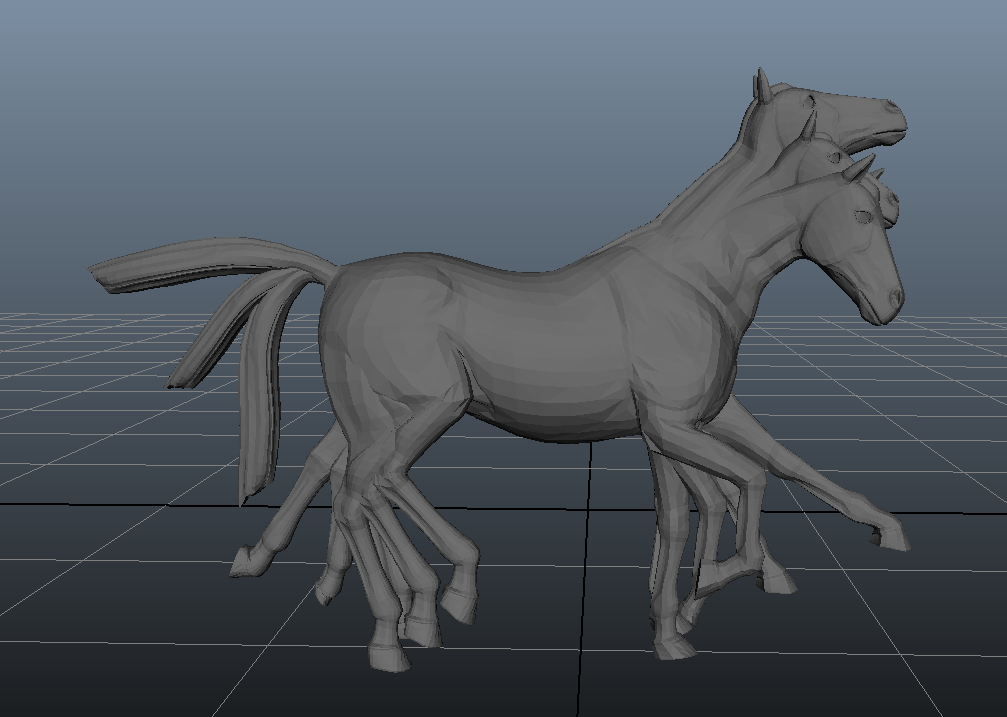
\includegraphics[width = 3in]{images/linearInterpolation1}}
\subfloat[fig 4]{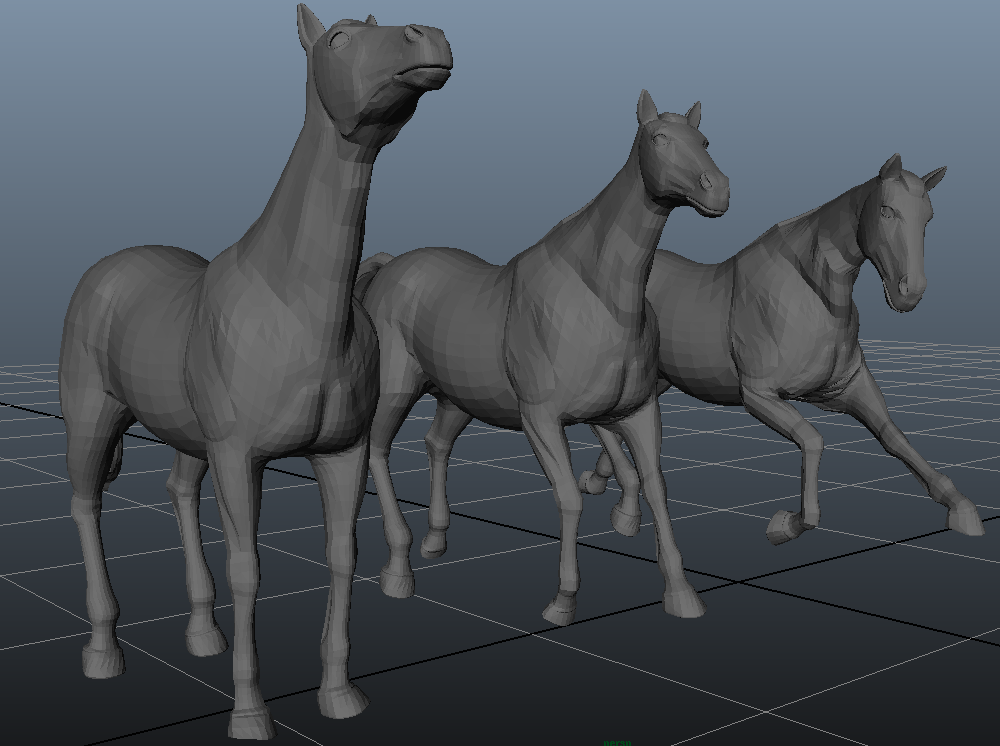
\includegraphics[width = 3in]{images/linearInterpolation2}}\\
\subfloat[fig 1]{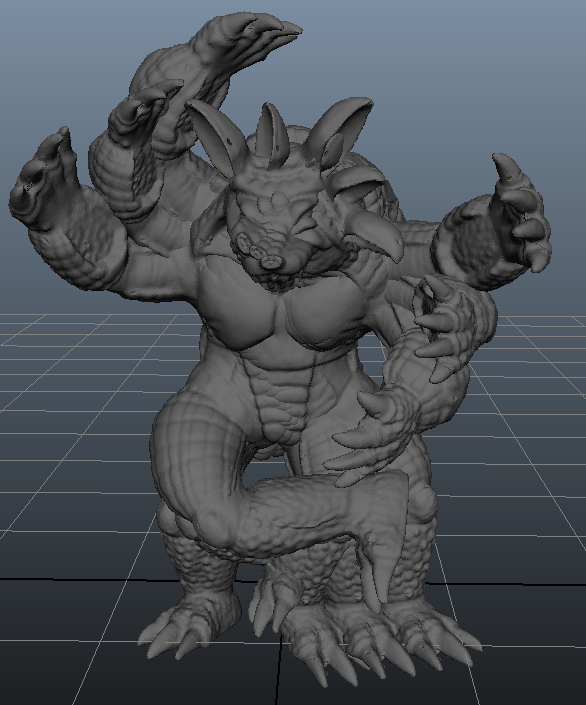
\includegraphics[width = 1.8in]{images/armadillo2}}
\subfloat[fig 2]{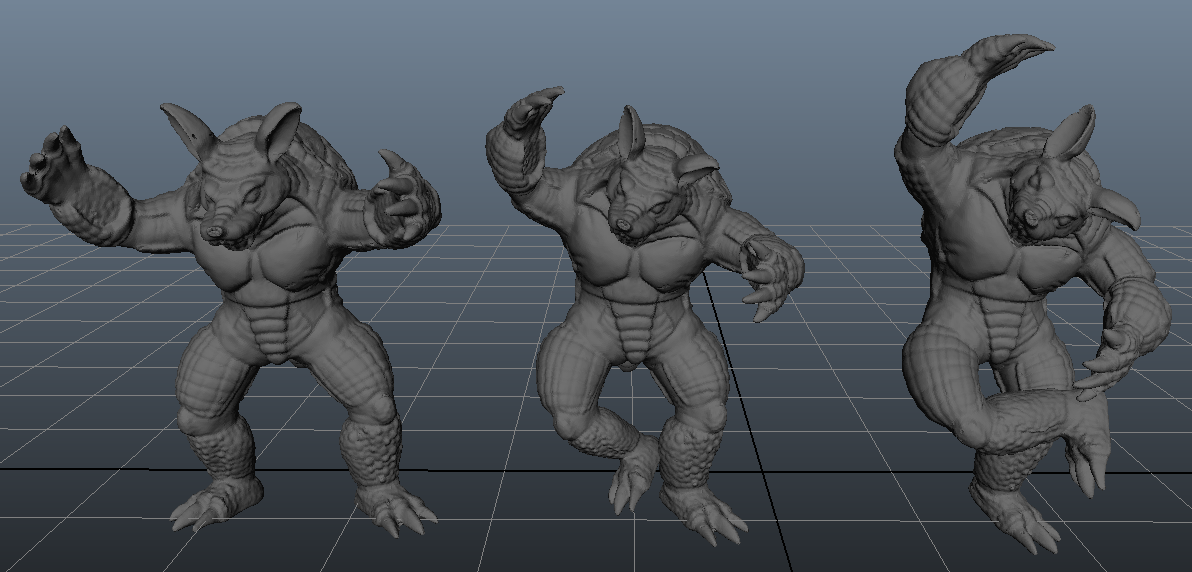
\includegraphics[width = 3.3in]{images/armadillo1}} 
\caption{Horse and armadillo meshes, morphed mesh is in the middle.}
\label{fig:linearInterpolation}
\end{figure}

\subsection{As rigid as possible interpolation}

The previous method produces distorted meshes due to its non-rigid nature.
One way to produce more better results is to use a transform-based technique.
Lets define an affine transformation from $\mathbf{p_i}$ to $\mathbf{q_i}$ such that:

\begin{align*}
A \mathbf{p_i} + \mathbf{l} = \begin{pmatrix}
 a_{11} & a_{12} & a_{13} \\ 
 a_{21} & a_{22} & a_{23} \\ 
 a_{31} & a_{32}  & a_{33} 
\end{pmatrix} 
\begin{pmatrix}
 p_{ix} \\ 
 p_{iy} \\ 
 p_{iz} 
\end{pmatrix} +
\begin{pmatrix}
 l_x \\ 
 l_y \\ 
 l_z
\end{pmatrix} = \mathbf{q_i},
\end{align*}

\end{document}

